\documentclass{article}
% translate with >> pdflatex -shell-escape <file>

% This file is an extract of the PGFPLOTS manual, copyright by Christian Feuersaenger.
% 
% Feel free to use it as long as you cite the pgfplots manual properly.
%
% See
%   http://pgfplots.sourceforge.net/pgfplots.pdf
% for the complete manual.
%
% Any required input files (for <plot table> or <plot file> or the table package) can be downloaded
% at
% http://www.ctan.org/tex-archive/graphics/pgf/contrib/pgfplots/doc/latex/
% and
% http://www.ctan.org/tex-archive/graphics/pgf/contrib/pgfplots/doc/latex/plotdata/

\usepackage{pgfplots}
\pgfplotsset{compat=newest}

\pagestyle{empty}

\begin{document}
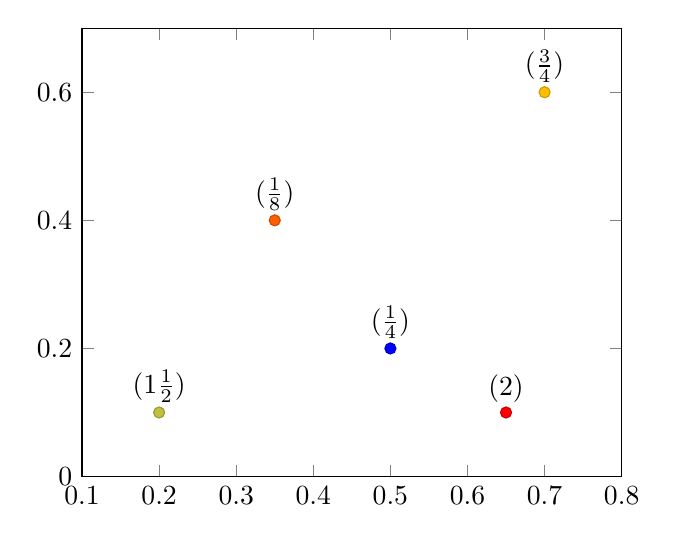
\begin{tikzpicture}
	\begin{axis}[enlargelimits=0.2]
		\addplot[
		  scatter,mark=*,only marks,
		  % we use 'point meta' as color data...
		  point meta=\thisrow{color},
		  % ... therefore, we can't use it as argument for nodes near coords ...
		  nodes near coords*={$(\pgfmathprintnumber[frac]\myvalue)$},
		  % ... which requires to define a visualization dependency:
		  visualization depends on={\thisrow{myvalue} \as \myvalue},
		] 
		table {
			x      y    color   myvalue
			0.5    0.2  1       0.25   
			0.2    0.1  2       1.5    
			0.7    0.6  3       0.75   
			0.35   0.4  4       0.125  
			0.65   0.1  5       2      
		};
	\end{axis}
\end{tikzpicture}
\end{document}
